\documentclass{standalone}

\usepackage{tikz}

\begin{document}
\begin{tikzpicture}

\definecolor{mc}{RGB}{214,39,40}

%defs für circle
\pgftext{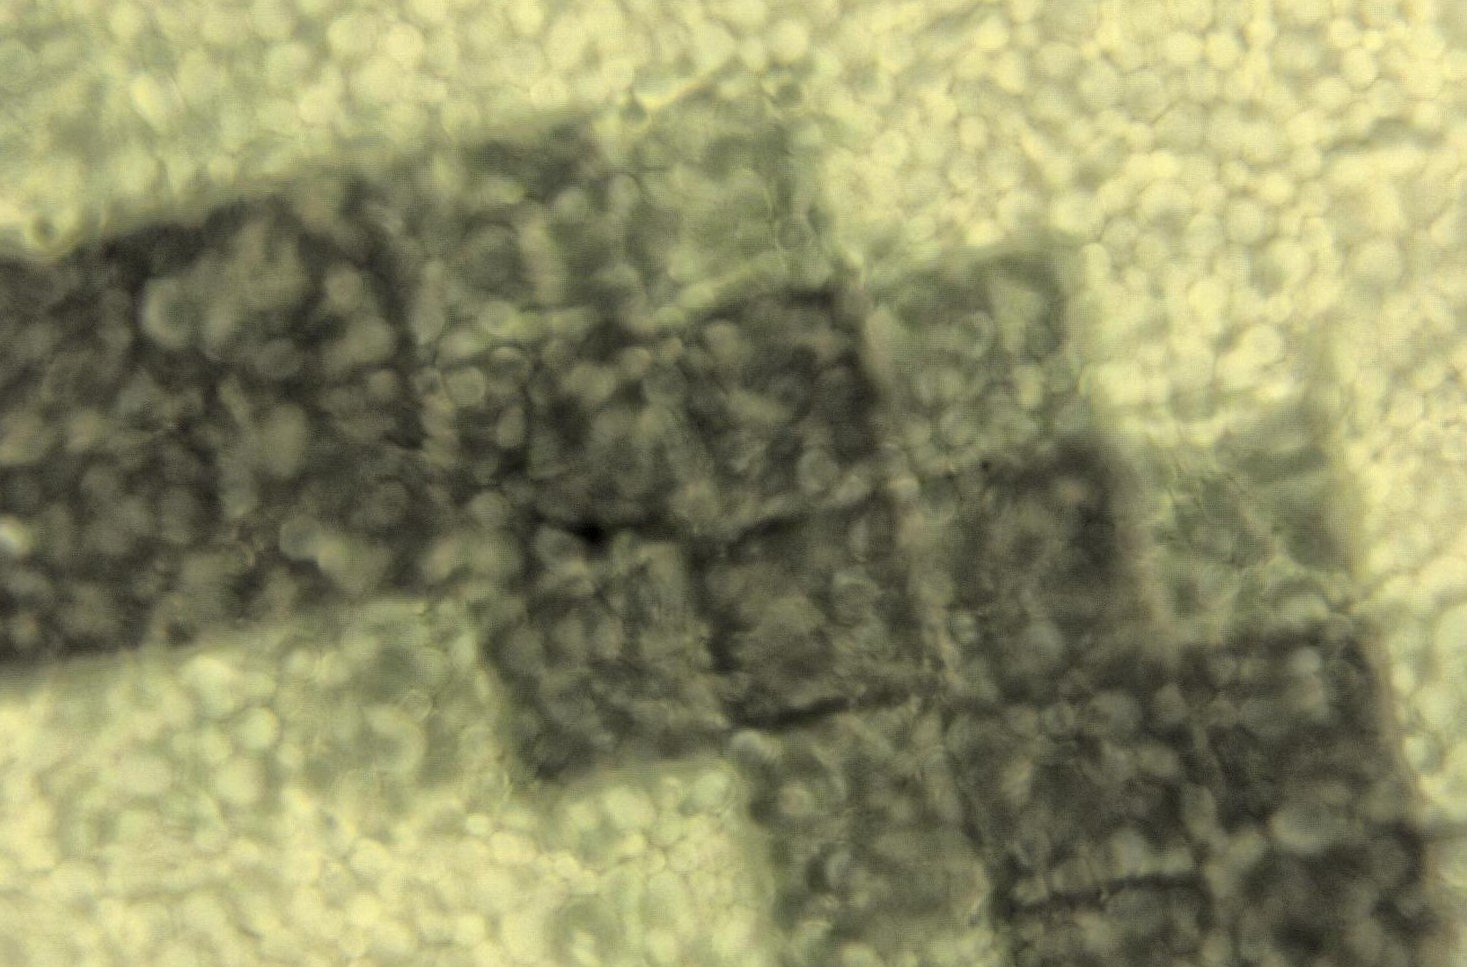
\includegraphics[width=600pt]{b.jpg}}
\def\C{3.24,0.84}
\def\R{0.33cm}
\def\TH{0.05cm}
\def\ANG{-12}
\tikzstyle{dashed}=[dash pattern=on 5pt off 5pt]


%defs für arrows
\def\ARR{4mm}	
\usetikzlibrary{arrows.meta}	
\tikzset{>={Latex[width=3mm,length=\ARR]}}

	
\draw[line width=\TH, mc, dashed] (\C) circle (\R);
	
\draw[-<, line width=\TH, mc] (\C) -- +(\ANG:\R+2*\TH+\ARR/2);
\draw[line width=\TH, mc] (\C) -- +(\ANG:1.1);
\draw[-<, line width=\TH, mc] (\C) -- +(\ANG+180:\R+2*\TH+\ARR/2);
\draw[line width=\TH, mc] (\C) -- +(\ANG+180:8.5);
\node[rotate=\ANG,font=\Huge, mc] at (-1.4,2.35) {0.02 mm - 0.04 mm};

\end{tikzpicture}
\end{document}